% Made up for the tikra benchmark.
\usetikzlibrary{circuits.logic.US, calc}
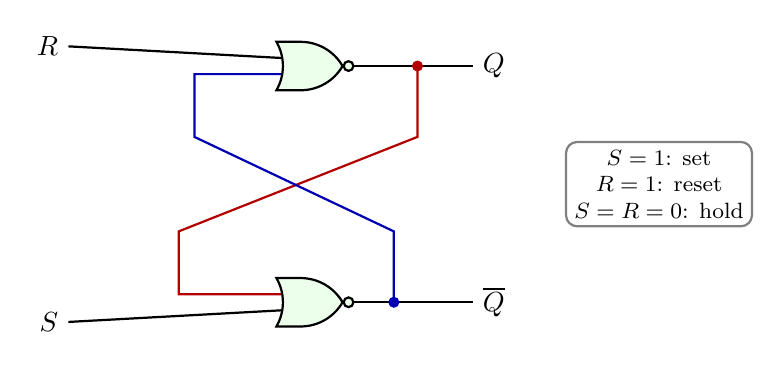
\begin{tikzpicture}[circuit logic US, thick, every circuit symbol/.style={fill=green!8}]
  \node[nor gate] (top) at (3,1.5) {};
  \node[nor gate] (bot) at (3,-1.5) {};
  \draw (0,1.75) node[left] {$R$} -- (top.input 1);
  \draw (0,-1.75) node[left] {$S$} -- (bot.input 2);
  \draw (top.output) -- ++(1.5,0) coordinate (q) node[right] {$Q$};
  \draw (bot.output) -- ++(1.5,0) coordinate (nq) node[right] {$\overline{Q}$};
  \draw[red!70!black] ($(top.output)+(0.8,0)$) -- ++(0,-0.9) -- (1.4,-0.6) |- (bot.input 1);
  \draw[blue!70!black] ($(bot.output)+(0.5,0)$) -- ++(0,0.9) -- (1.6,0.6) |- (top.input 2);
  \fill[red!70!black] ($(top.output)+(0.8,0)$) circle (2pt);
  \fill[blue!70!black] ($(bot.output)+(0.5,0)$) circle (2pt);
  \node[font=\footnotesize, align=center, draw=gray, rounded corners, inner sep=3pt]
    at (7.5,0) {$S=1$: set\\$R=1$: reset\\$S=R=0$: hold};
\end{tikzpicture}
